\documentclass[
oneside, % Хоёр талаар хэвлэж үдэхээр тохируулсан. Нэг тал бол комментыг арилга
%chapterinoneline,% Нэг мөрөнд бүлгийн дугаар, нэрийг гаргах
english, % babel багцын хэлний тохиргоо
onehalfspacing, % Мөр хоорондын зай. Сонголтууд: singlespacing, onehalfspacing, doublespacing
%draft, % Ноорог горимд шилжихийн тулд комментыг ар	илга(зураг, холбоос, hboxes гарахгүй)
nolistspacing, % Хэрэв мөр хоорондын зай onehalfspacing эсвэл doublespacing бол, жагсаалтын мөр хоорондын зайг single болгохын тулд комментыг арилга
%liststotoc, % Зураг/хүснэгт/бусад жагсаалтыг гарчигт оруулахын тулд комментыг арилга
%toctotoc, % Uncomment to add the main table of contents to the table of contents
%parskip, % Параграф хооронд зай оруулахын тулд комментыг арилга
%nohyperref, % hyperref багцыг ачаалахгүй бол комментыг арилга
headsepline, % Толгой мөрийн доогуур шугам татахын тулд комментыг арилга
]{article} % Энэ класс файл нь баримтын бүтцийг тодорхойлно

\usepackage[utf8]{inputenc}
\usepackage[T2A]{fontenc}
\usepackage[mongolian]{babel}
\usepackage{graphicx}
\usepackage{titlesec}
\usepackage{./thesis}
\graphicspath{ {images/} }
\begin{document}
\thesistitle
	{ Оюутны онлайн сургалтын системийн бичиг баримт}
	{\emph{ Н. Алтаночир\\B150920063@mymust.net}}
	{\emph{''Мэдээллийн системийн''}}
	{\emph{ Мэдээлэл Холбоо Технологийн Сургууль}}
	{\emph{2018-11-28}}
	
	
    \tableofcontents
   
	\section{Оршил}
	   
	   Их сургуулийн олон нийтийн сүлжээний хэрэглэгчийн бүртгэлийн систем нь хэрэглэгчиддээ бүртгэх оюуны өмчийг хамгаалах, мэдээлэлийг хэрхэн авах, гаргах зэрэг дээр хүндрэлтэй байдаг тул энэ үйл ажиллагаануудыг хялбарчлахад чиглэсэн.
	   
	\subsection{Системийн зорилго}
	• Багш бүр хичээлийн дүнгээ нэг бүчлэн өөрийн хүссэнээр даалгавар нэмэж хасаж бүртгэх боломжой.
	\subsection{Системийн хүрээ хязгаар}
	•Их сургуулийн олон нийтийн сүлжээн, оюутны moodle систем.
	\subsection{Нэр томъёоны тайлбар}
	• grade - дүн (англи нэр)
	\section{Судалгаа}
	\subsection{Програмын судалгаа}
	\subsubsection{Монголын  системүүдийн харьцуулсан судалгаа}

	\begin{itemize}
	\item  Улирлын жилийн эцсийн дүн хичээлийн явцыг удирдах сурагч болон эцэг эхчүүдийн системд нэвтрэх эрхийг үүсгэх боломжтой.Удирдсан ангийн сурагчдын мэдээлэлтэй ажиллах, ангийн хичээлийн хуваарь, ирцийн мэдээлэл, сургалтын мэдээлэл, ангийн журнал харах, тайлан гаргах, ангийн сурагчийн жилийн эцсийн тодорхойлолт, ангийн дүнгийн хавтгай гаргах боломжтой. Мөн өөрийн сургалтын мэдээлэл харах, өөрийн ирцийн мэдээлэлтэй танилцах, өөрийн хичээлийн хуваарь харах, заасан хичээлийн тэмдэглэл хөтлөх, заадаг ангийн сурагчдийн дүн, ирцийн мэдээлэл оруулах, ерөнхий тайлан гаргах зэрэг үйлдлүүдийг хийж блно.лирлын жилийн эцсийн дүн хичээлийн явцыг удирдах сурагч болон эцэг эхчүүдийн системд нэвтрэх эрхийг үүсгэх боломжтой.
	\item Эцэг эхчүүд нь  багш, сургууль байнгын холбоо харилцаатай байх боломжтой  бөгөөд хүүхдийнхээ хичээлд оролцсон байдал ирц, хичээлийн хуваарь, болон бусад мэдээллүүдтэй танилцах, заасан хичээлүүдийн хөтөлбөрийг нь харах боломжтой юм.
	
	\subsubsection{ТЭЭВРИЙН ДЭЭД СУРГУУЛЬ оюутны веб}
	\item Эцэг эхчүүд  хүүхдийнхээ  хичээлийн оролцоо дүнг мэдээлэл авах,хянах боломжтой
	\item Сурагч хичээлийн хуваарь, дүнгийн мэдээлэл  явцын дүн мэдэх боломжтой

	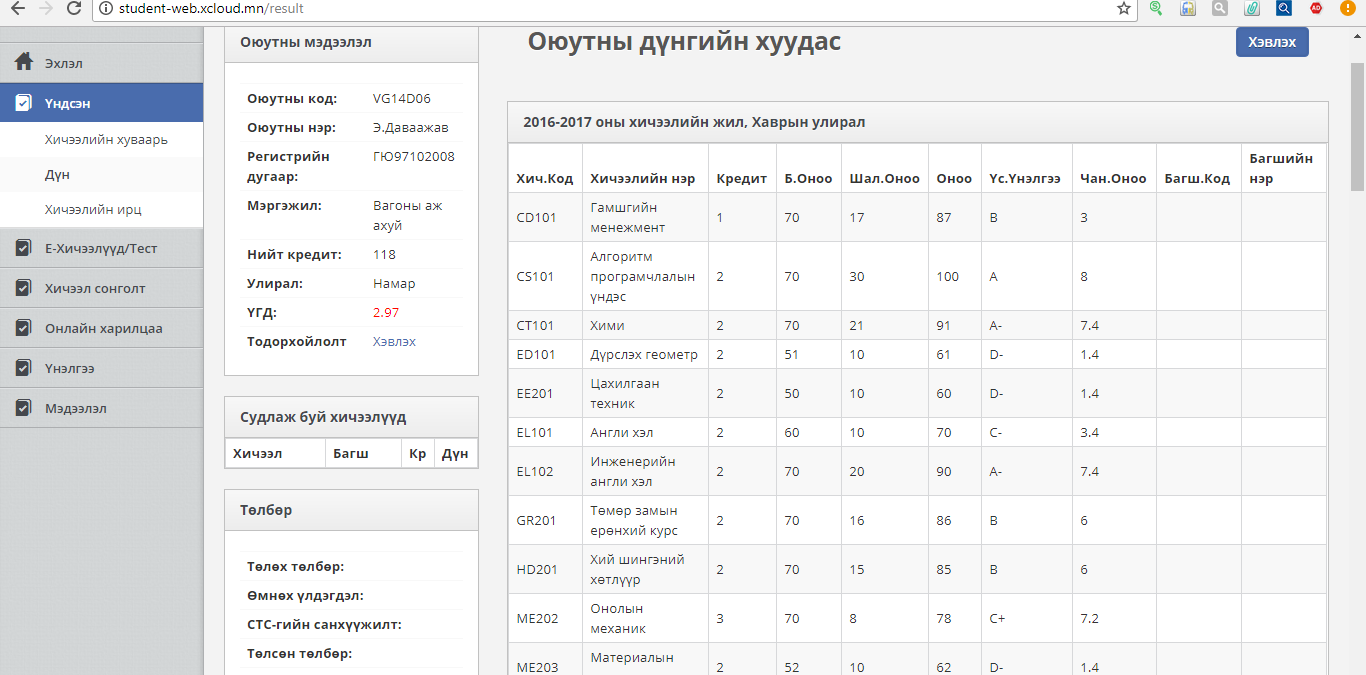
\includegraphics[width=\textwidth]{zurag}
\end{itemize}

	\subsection{Гадаад facebook системтэй харьцуулсан судалгаа}
	
	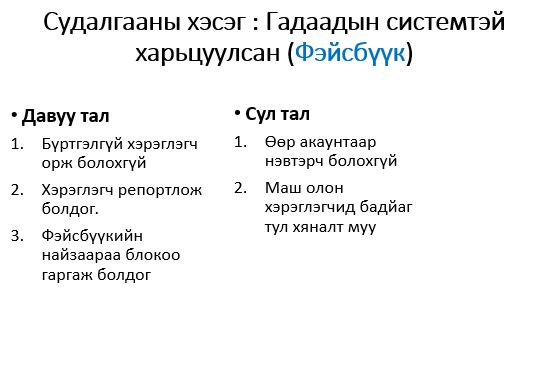
\includegraphics[width=\textwidth]{gadaadsudalgaa}

	
	\subsection{Хууль, дүрэм журам}
	2010 онд БСШУ-ны Сайдын 2007 оны 6 дугаар сарын 5-ны өдрийн 183 тоот тушаалын 6 дугаар зүйлд заасны дагуу дотоодын их сургууль, коллежийн зайн сургалт явуулж болно. 
	
	
	\section{Технологийн судалгаа}
	
	\subsection{MySQL}
	MySQL нь холбоост өгөгдлийн санг удирдах систем юм. MySQL хэмээх нэрний хувьд уг системийг санаачлан хөгжүүлэгч Micheal Widenius-ын охины нэр My + SQL(Structed Query Language) гэсэн утгатай ажээ.
	Энэ систем нь GNU (General Public License) буюу нээлтэй эхийн систем учир хүссэн хэн бүхэн хөгжүүлэлтэнд оролцож, үнэгүй хэрэглэж болох юм. Эзэмшигч нь алдарт Java-г хөгжүүлсэн Sun MicroSystems компани байсан ба, одоогоор Sun-г Oracle корпораци эзэмших болсон билээ.
	Үнэгүй програм хангамжийн өгөгдлийн санг удирдах системд ихэвчлэн MySQL-ийг хэрэглэдэг бөгөөд тэдгээрийн сонгодог жишээ гэвэл Joomla, Drupal, Wordpress, phpBB гэх мэт агуулга удирдах системүүд (CMS-Content Management System), Wikipedia, Facebook, Google гэх мэт томоохон компаниуд хэрэглэдэг юм.
	Хөгжүүлэлт нь C/C++ хэл дээр хийгдсэн ба AIX, BSDi, FreeBSD, HP-UX, i5/OS, Linux, Mac OS X, NetBSD, Novell NetWare, OpenBSD, OpenSolaris, eComStation, OS/2 Warp, QNX, IRIX, Solaris, Symbian, SunOS, SCO OpenServer, SCO UnixWare, Sanos, Tru64, Microsoft Windows гэсэн олон үйлдлийн системүүд дээр ажилладаг.
	MySQL бол хамгийн өргөн хэрэглээтэй нээлттэй эхийн (Open Source) өгөгдлийн сан удирдах програм юм. Анх 1995 онд зах зээлд гарсан ба с/с++ хэл дээр бичигдсэн. Одоогийн байдлаар 5.7 нь хамгийн сүүлийн хувилбар болон гараад байна. Энэ сүүлийн хувилбар дээр нэмэгдсэн давуу талууд гэвэл 3 дахин хурдан үйл ажиллагаатай болсон мөн натив JSON дэмжигчтэй болсон гэх мэт шинэлэг үйлдлүүд нэмэгдсэн байна.
	
	\subsection{Php}
	Rasmus Lerdorf WWW-д вэб хуудас үүсгэх үедээ өгөгдөл боловсруулах хялбархан арга хайж байгаад 1995 онд PHP хэлийг скрипт хэл байдлаар зохиосон.
	PHP нь сервер талын скрипт хэл ба динамик вэб хуудас хийхэд илүү тохиромжтой. Энэ скрипт хэл нь энгийн хэрэглээний вэб сайтаас эхлээд байгууллагын иж бүрэн вэб программ хийж болохоор MySQL мэтийн өгөгдлийн сантай харилцан ажиллах боломжтой.
	Хуудас ачаалах үед броузерээр нэг бүрчлэн уншдаг HTML-тэй адилгүй, PHP баримтыг бэлтгэхдээ серверээр урьдчилан боловсруулдаг. PHP код агуулсан хуудас нь хэрэглэгчийн броузерт илгээгдхээс өмнө серверээр боловсруулагдсан байдаг.
	PHP хэлний өөр нэг давуу тал бол скриптэн хэл юм. Ихэнх програмчлалын хэлнүүдэд ажиллахын өмнө машины хэл рүү хөрвүүлэх тусгай файлууд /compile/ шаардлагатай байдаг бол PHP хэлний хувьд хөрвүүлэлт хийх шаардлагагүй байдаг тул код засварлах болон шалгахад илүү хурдан байдаг
		
		\subsection{Эрхийг өргөжүүлэх (privilege escalation) халдлага гэж юу вэ? }	
		Privilege escalation буюу эрхийг өргөтгөх нь аюултай аюул ганал юм. 
		Privilege escalation-ийн боломжоос хамааран хортой нэмэлт нэмэх, өгөгдлийн өөрчлөх, устгах боломж олгож байгууллагыг хүнд бадйлд сүрэлд оруулдаг юм.
		
		
	\newpage
	\section{Шинжилгээ, зохиомжийн хэсэг}
	\subsection{Функциональ шаардлага}
	\paragraph {Багш}
     \begin{itemize}
 	
 	\item Хичээлийн жагсаалт харах ( Өөрийн орж байгаа )
 	\item Тухайн хичээл заалгуулж байгаа оюутнуудыг харах
 	\item Оюутны дүнг оруулах
 	\item Оюутны дүнг засах
 
 	
    \end{itemize}
	\subsection{Функциональ бус шаардлага}
	\begin{itemize}
		\item Хэрэглэхэд хялбар ойлгомжтой, дэлгэрэнгүй байх
		\item Мэдээллийг түргэн шуурхай харуулдаг байх
		\item Алдааны мэдээлэл өгдөг байх 
		\item Бүх төрлийн төхөөрөмжид тохиромжтой хэлбэрээр харагддаг /респонсив/ загвартай байна
	\end{itemize}
	\section{Юзкейс диаграм}
     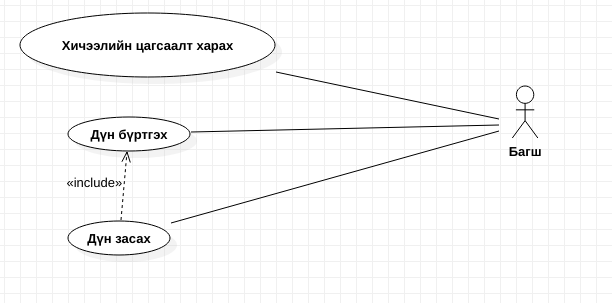
\includegraphics[width=\textwidth]{bagsh}
     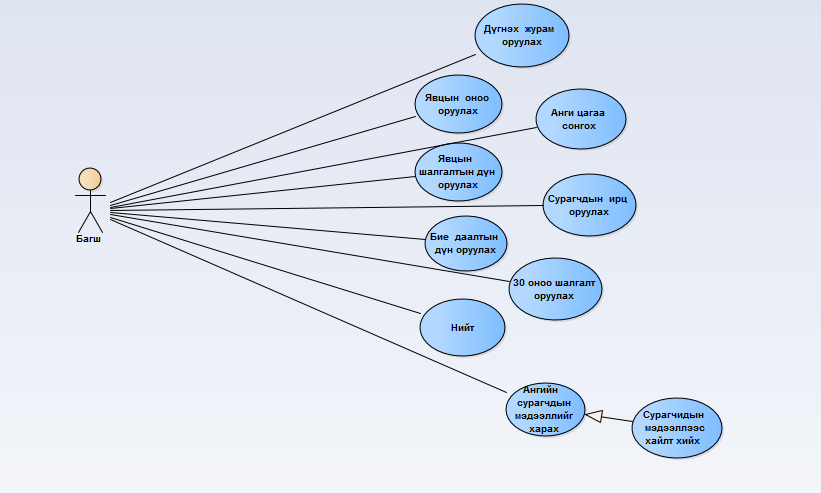
\includegraphics[width=\textwidth]{Usecase2}
     	\subsection{Хичээлийн жагсаалт интерфэйс}
     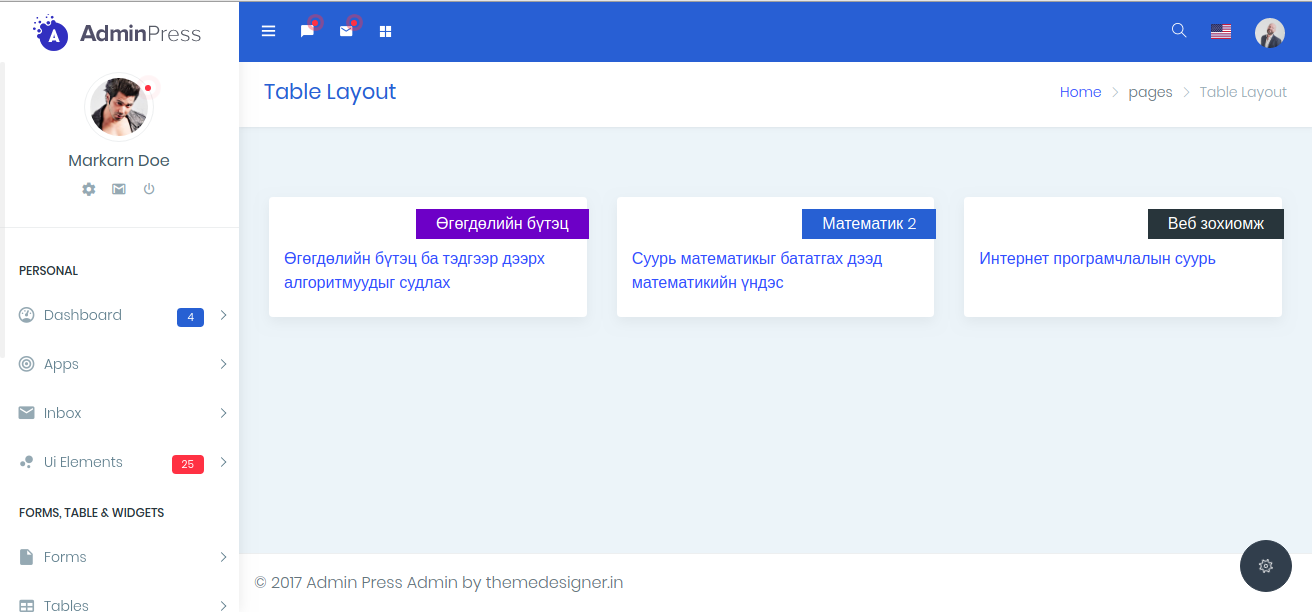
\includegraphics[width=\textwidth]{course_list}
     \subsection{Дүнгийн интерфэйс}
     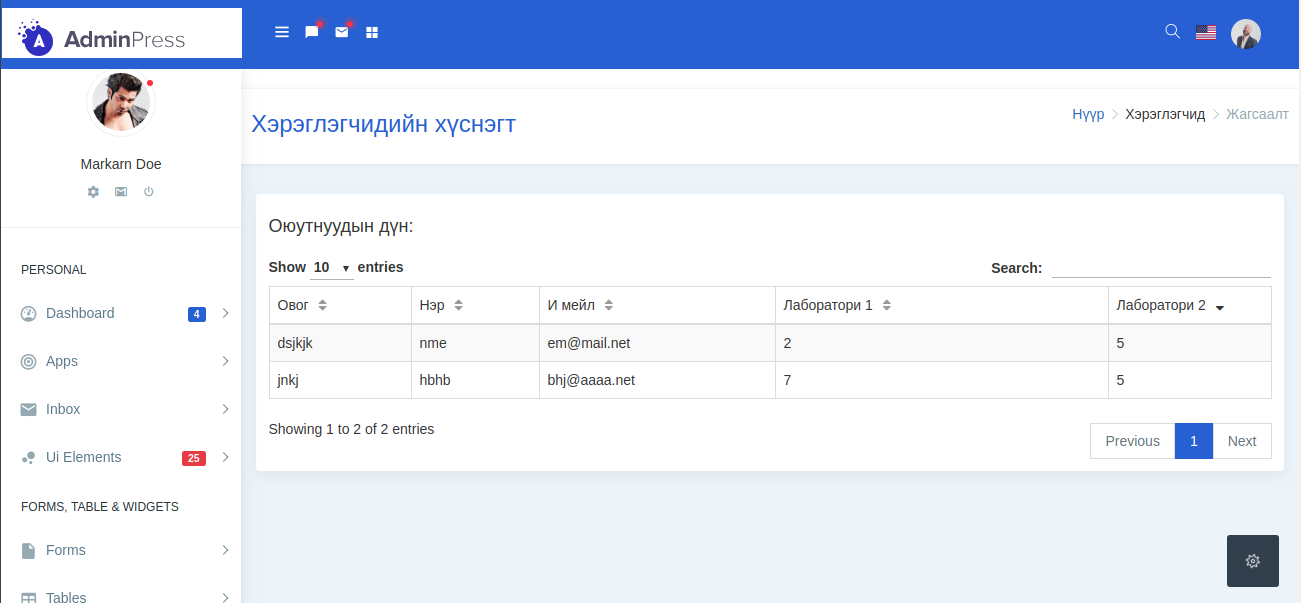
\includegraphics[width=\textwidth]{dvn}
     	
     	\section{Үйл ажиллагааны диаграм}
     	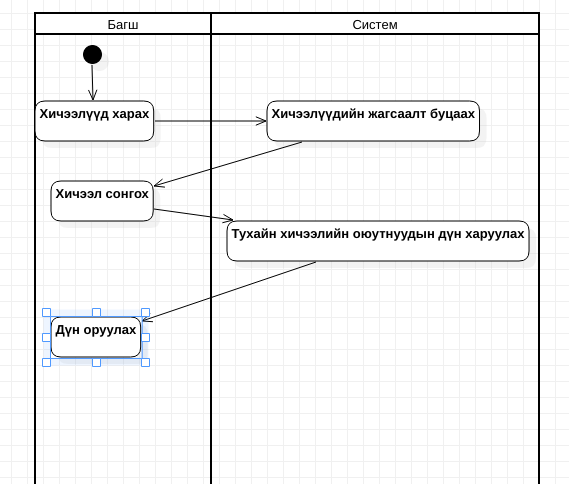
\includegraphics[width=\textwidth]{dvnoruul}
     	
     \section{Обьектын холбоосын диаграмм ( ERD )}
     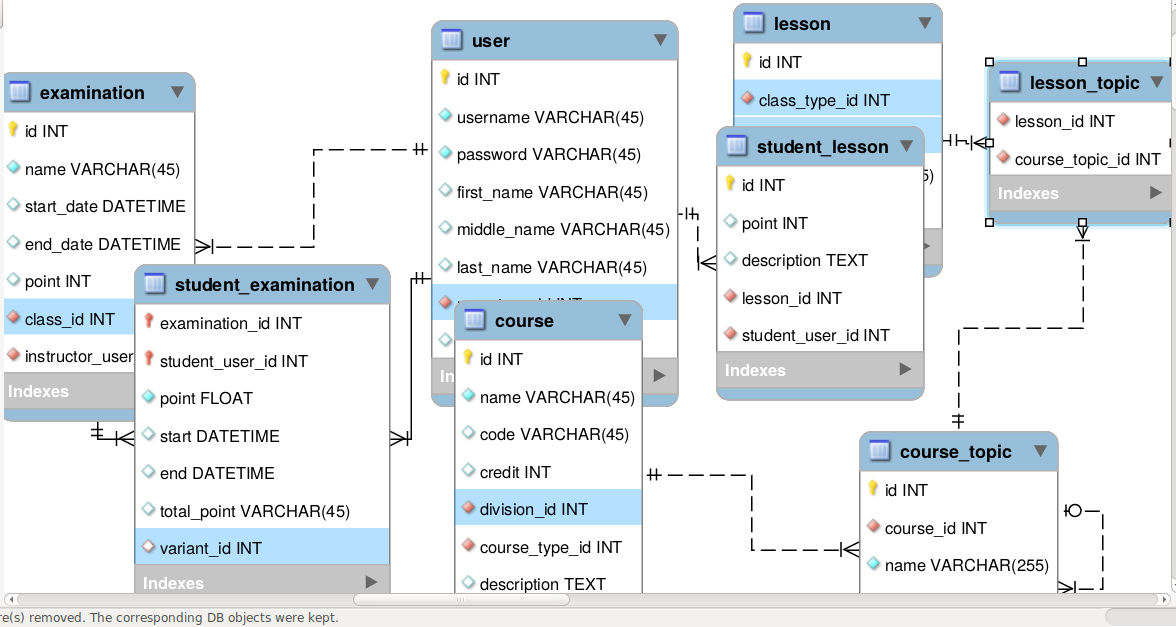
\includegraphics[width=\textwidth]{erd}
      \section{Класс диаграм ( Class diagram )}
     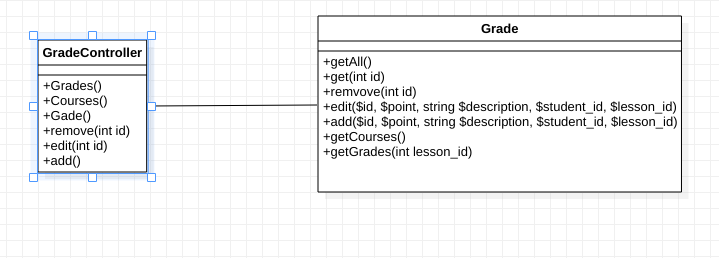
\includegraphics[width=\textwidth]{cdiagram}
     \section{Дараалалын диаграмм( Sequence diagram )}
     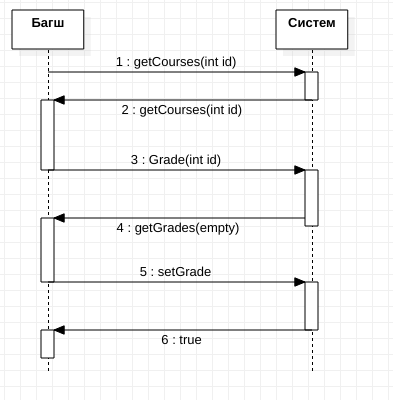
\includegraphics[width=\textwidth]{activityd}
     
      \section{Төлөвийн диаграм }
     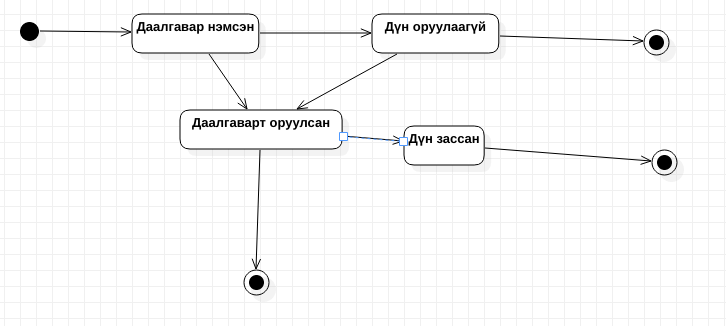
\includegraphics[width=\textwidth]{stated}
     
     \section{Тестын зохиомж }
      \subsection{ Хичээлийн жагсаалт харах }
     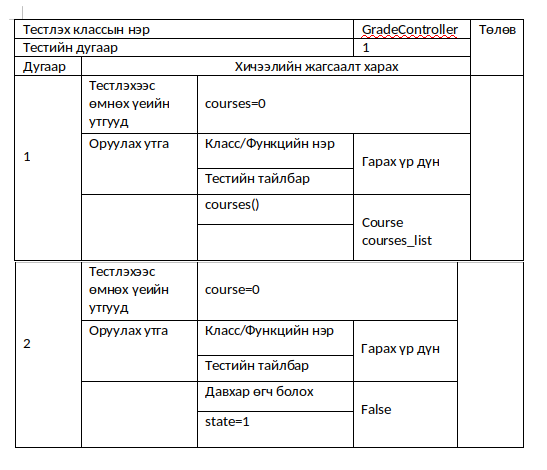
\includegraphics[width=\textwidth]{hihi}
      \subsection{Дүн нэмэх}
     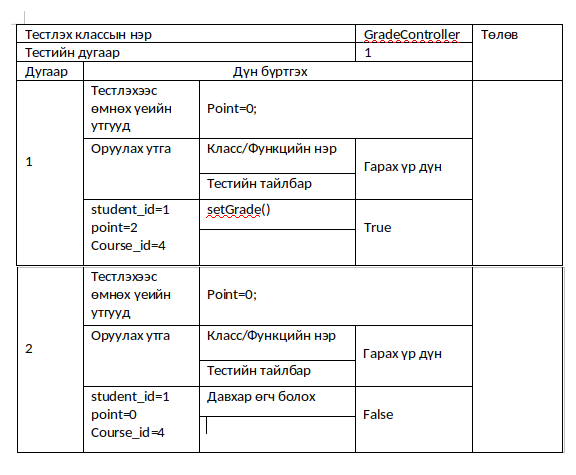
\includegraphics[width=\textwidth]{hihi1}
     
     \section{Дүгнэлт}
     Хамгийн гол нь дүнгийн бүртгэл хурдан шуурхай ойлгомжтой яг excel дээр хийж байгаа шиг бүтээмжтэй байх бөгөөд загвар үзэмжийн хувьд илүү сайн байх.
    
     
     \section{Ашигласан бүтээлийн жагсаалт}
     \subsection{Ном зүй}
     \subsection{Вэб сайтууд}
     http://www.schoolweb.mn/schools/
     
     http://www.meds.gov.mn/data/said/Боловсрол%20Эрх%20зүйн%20баримт%20бичиг.pdf
     
\end{document}



